%!TEX root=dissertation.tex
\chapter{Типовой канал волоконного лазера киловаттного уровня на собственной элементной базе}
\label{chapt4}

\section{Введение}
\label{sec:kw-intro}

Разработка мощных волоконных лазеров является актуальной задачей, поскольку такие лазеры находят широкое применение в научных исследованиях и в промышленности для обработки материалов. В последнем случае привлекательными являются лазеры мощностью более 5~кВт с высоким качеством излучения.

Масштабирование мощности волоконных лазеров ограничено рядом физических факторов, обозначенных в отчете [1]. Основными ограничивающими факторами являются оптический пробой и нелинейные эффекты, пороги возникновения которых, в основном зависят от длины волокна и диаметра сердцевины.

Наиболее высоким качеством излучения в сочетании с высокой мощностью обладают лазеры с диаметром сердцевины 20-25~мкм. Согласно [1], при диаметре сердцевины 20~мкм теоретически возможно достичь мощности порядка 6~кВт в одноволоконном исполнении (без сложения излучения нескольких лазеров). Дальнейшее увеличение мощности может приводить к развитию нелинейных эффектов и оптическому пробою.

Тем не менее, чтобы достичь мощности порядка 6~кВт в одноволоконном исполнении необходимо как минимум 8~кВт излучения накачки (при эффективности <<свет в свет>>~75~\%). На сегодняшний день коммерчески доступных объединителей накачки, способных выдержать такую мощность, нет. Другим способом ввода излучения накачки в активное волокно является использование GTWave технологии, когда в одном волокне расположены световоды излучения накачки и активный световод. На данный момент во ВНИИТФ и в России нет отработанной технологии изготовления подобного волокна.

Поэтому достижение мощности более 5~кВт видится путем объединения излучения лазерных модулей с максимально возможной на данный момент мощностью. Кроме того модульность конструкции позволит в дальнейшем получать мощности более 10~кВт в частности 100~кВт и выше. Но в этом случае нужно помнить, что качество излучения будет ниже, чем в одноволоконном исполнении.
В настоящей работе будут представлены результаты разработки и создания лабораторного образца оптоволоконного лазера с мощностью излучения 5~кВт с применением модульной конструкции.

\section{Оптическая схема лазера}
\label{sec:kw-scheme}

\subsection{Оптическая схема задающего генератора}

Оптическая схема задающего генератора представлена на рисунке 1.
\begin{figure}
  \centering
  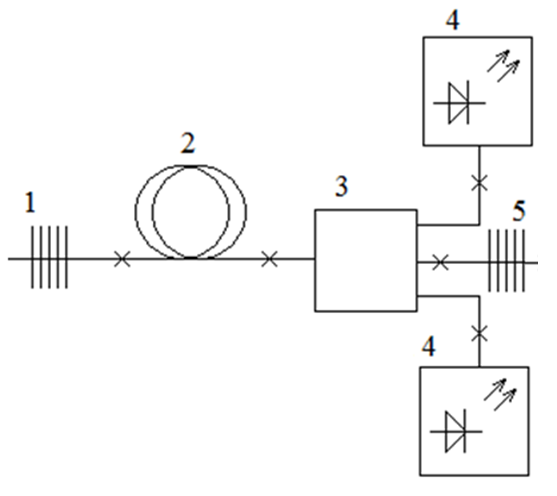
\includegraphics[scale=0.6]{kw-1}
  \caption{Оптическая схема задающего генератора: 1 – глухая решетка; 2 – активное волокно; 3 о–бъединитель накачки; 4 – модуль накачки; 5 – выходная решетка.}
  \label{img:kw-1}
\end{figure}

Для накачки активного волокна (4) используются модули накачки мощностью 30~Вт в количестве 2 шт. производства ВНИИТФ. Для ввода накачки в активное волокно используется объединитель типа (2+1)х1 суммарной поддерживаемой мощностью 100~Вт (Lightcomm). Объединитель имеет два многомодовых входа с параметрами волокна 105/125~мкм и NA = 0,22, сигнальное волокно имеет параметры 10/125~мкм и NA = 0,08. Глухая брэгговская решетка (1) имеет коэффициент отражения 99~\% на длине волны 1080~нм, а выходная (5) около 5~\% (нужна эта решетка для формирования резонатора, т.к. при сварке с усилителем обратная связь в задающем генераторе будет отсутствовать), выбирается оптимальной из расчета и экспериментальной отработки.

\subsection{Оптическая схема волоконного усилителя}

Оптическая схема мощного волоконного усилителя представлена на рисунке 2.
\begin{figure}
  \centering
  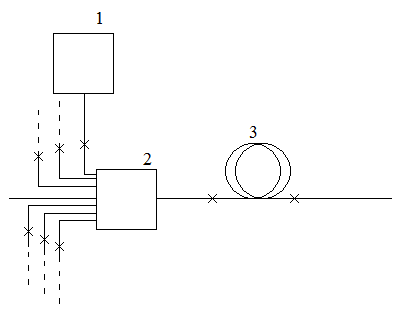
\includegraphics[scale=0.6]{kw-2}
  \caption{Оптическая схема волоконного усилителя: 1 – система объединения накачки; 2 – объединитель накачки (6+1)х1; 3 – активное волокно; х – места сварки.}
  \label{img:kw-2}
\end{figure}
Для накачки активного волокна (3) используются модули накачки мощностью 30~Вт в количестве 36 шт. производства ВНИИТФ. Для ввода накачки в активное волокно используется объединитель типа (6+1)х1 суммарной поддерживаемой мощностью 1200~Вт MMC0611C3553 (ITF Labs, либо аналог Lightcomm). Объединитель имеет шесть многомодовых входов с параметрами волокна 200/220~мкм и NA = 0,22, сигнальное волокно на входе 10/125~мкм и NA = 0,08/0.46, на выходе - 20/400~мкм и NA = 0.06/0.46. Поскольку модули накачки имеют выходное волокно с параметрами 105/125~мкм и NA = 0,15, то для стыковки с каплером (6+1)х1 они объединяются каплером 7х1 с параметрами входных волокон 105/125 NA = 0,15 и выходным - 200/220 NA = 0,22. Система объединения накачки представлена на рисунке 3.
\begin{figure}
  \centering
  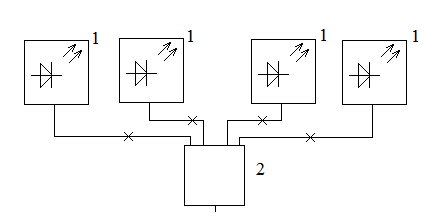
\includegraphics[scale=0.6]{kw-3}
  \caption{Система объединения накачки каплером типа 7х1 (на рисунке только 4 канала): 1 – модуль накачки; 2 – объединитель накачки.}
  \label{img:kw-3}
\end{figure}

Если считать эффективность объединения накачки 95~\% и эффективность преобразования <<свет в свет>> 70~\%, то на выходе ЗГ мощность лазерного излучения должна составлять примерно 40~Вт, а после усиления 760~Вт. При сложении семи таких модулей общая выходная мощность должна составлять более 5~кВт.

\section{Моделирование волоконного лазера}
\label{sec:kw-modeling}

На рис. 1 приведена стандартная схема волоконного лазера с распределенной накачкой.

\begin{figure}[ht]
  \centering
  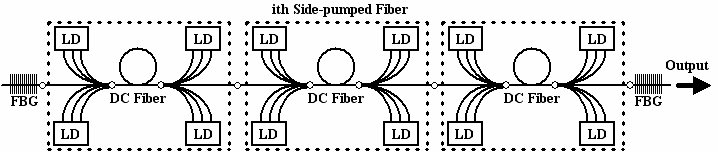
\includegraphics[scale=0.6]{laser_vlrn_1}
  \caption{Структура волоконного лазера с распределенной накачкой.}
  \label{img:laser_vlrn_1}
\end{figure}

Лазер созданный по схеме ВЛРН имеет ряд преимуществ по сравнению с классической схемой MOPA:
\begin{enumerate}
  \item Более равномерное распределение тепловых нагрузок вдоль волокна.
  \item Большее число мест ввода накачки позволяет использовать модули накачки меньшей мощности при одинаковой выходной мощности.
  \item При достаточной оптимизации конструкции лазера возможна определенная масштабируемость.
  \item Более высокая расчетная эффективность лазера по сравнению со схемой MOPA.
\end{enumerate}

Для оценки выходной мощности волоконного лазера с распределенной накачкой (ВЛРН) была написана программа в среде Matlab для решения системы обыкновенных дифференциальных уравнений (система уравнений связанных волн и стационарный случай скоростных уравнений) вида [14]:

(1)

(2)

(3)

(4)

(5)

В приведенных соотношениях использованы следующие обозначения: $z$ – координата по длине световода, $N_2$ и $N$ -- населенность метастабильного уровня и общая концентрация ионов иттербия, соответственно. $P_p, P_s$ -- мощности накачки и сигнала, соответственно. Для усиленной спонтанной люминесценции знаки плюс и минус означают направление распространения. $\tau$ -- время жизни на метастабильном уровне, для распространенных составов стекла оно составляет 10-13 мс. $\sigma_{as}$ и $\sigma_{es}$ -- сечения поглощения и эмиссии на длине волны усиливаемого сигнала, $\sigma_{ap}$ и $\sigma_{ep}$ -- сечения поглощения и эмиссии на длине волны накачки. $\Gamma_p$ -- фактор перекрытия излучения накачки с сердцевиной, $\Gamma_s$ -- фактор перекрытия излучения генерации с сердцевиной. $А$ -- эффективная площадь сердцевины, $\alpha_p$ и $\alpha_s$ -- отношения сечений поглощения и эмиссии на длине волны накачки и генерации соответственно. $h\nu$ -- энергия фотона.

Решение системы уравнений должно удовлетворять ряду граничных условий. В нашем случае четырехсекционный волоконный лазер с распределенной накачкой имеет участки длиной $L_1, L_2, L_3$ и $L_4$. На концах каждой секции располагаются (привариваются) каплеры для ввода накачки в точках $L_{i1}$, $L_{i2}$ ($i$ обозначает номер секции), которые обеспечивают накачку величиной $P^+_p(L_{i1})$ и $P_{p}^{-}(L_{i2})$ в прямом и обратном направлениях соответственно. Мощность модулей накачки составляет $P_{i1}$ и $P_{i2}$. Длина каждой секции активного волокна выбрана достаточной, чтобы не учитывать потерю накачки на соседнем каплере (непоглощённая накачка). Граничные условия для $P_{p}^{+}(z)$ и $P_{p}^{-}(z)$ выглядят следующим образом:

(6)

(7)

где $\eta_2$ -- потери при вводе накачки (эффективность ввода накачки) через каплер. $P_s^{+}(z)$ и $P_s^{-}(z)$ связанны через коэффициенты отражения $R_1$ и $R_2$, что представляет собой стандартные граничные условия для линейного резонатора. Кроме того, функции $P_s^{+}(z)$ и $P_s^{-}(z)$ должны быть непрерывны на границе секций с учетом потерь $\eta_1$ на сварке секций. Таким образом, граничные условия для $P_s^{+}(z)$ и $P_s^{-}(z)$ можно записать как

(8)

(9)

(10)

(11)

Все использованные в расчете параметры и их значения приведены в таблице 1.

Таблица 1. Значения параметров, использованных в расчете ВЛРН [14].

В среде Matlab решение системы уравнений (1-5) с граничными условиями (6-11) можно выполнить двумя способами: 1 – с помощью встроенной процедуры решения системы обыкновенных дифференциальных уравнений с граничными условиями bvp4c; 2 – с использованием крайне популярного при расчете мощности волоконных лазеров метода <<simple shooting>>.

\textbf{Метод bvp4c}

График распределения мощности сигнала и накачки в прямом и обратном направлениях вдоль волокна, рассчитанный с использованием встроенной функции bvp4c, приведен на рис. 2. Следует отметить, что данный метод расчета, несмотря на свою простоту реализации, имеет один существенный недостаток. Для выполнения расчета необходимо предоставить ряд существующих решений всех искомых функций в некоторой точке. В данном случае выбор подобных решений носит эвристический характер. Подобный метод расчета лучше всего проводить при наличии экспериментальных результатов, получение которых, как правило, крайне затруднительно.

\begin{figure}[ht]
  \centering
  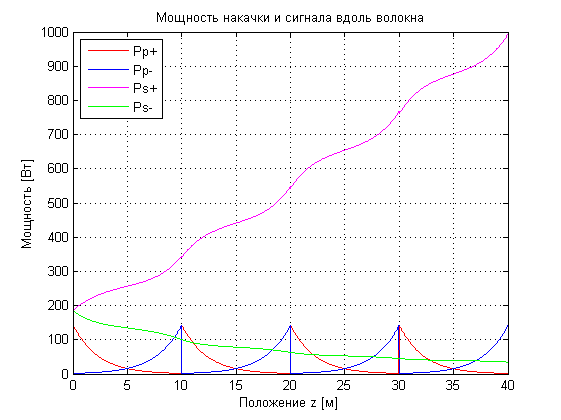
\includegraphics[scale=0.6]{laser_vlrn_2}
  \caption{Мощность накачки и сигнала как функции положения вдоль волокна, рассчитанные с помощью процедуры mathlab bvp4c.}
  \label{img:laser_vlrn_2}
\end{figure}

Тем не менее, полученный результат при соответствующем выборе опорных решений (guess) согласуется с результатами работы [14].

\textbf{Метод <<simple shooting>>}

Будем решать систему уравнений (2-5) методом Рунге-Кутты (функция ode45 в Matlab). Начальное значение $P_p^{+}(0)$ известно из (6). Неизвестные начальные условия для $P_p^{-}(0)$ и $P_s^{+}(0)$ будем искать методом <<simple shooting>>. В первом случае мы будем искать в цикле такое значение $P_p^{-}(0)$, чтобы $P_p^{-}(L)$ было равно известному нам значению (7). При достижении заданной величины ошибки (точности) значение $P_p^{-}(0)$ будет считаться найденным. Во втором случае все обстоит несколько сложнее. В этом случае неизвестно ни начальное, ни граничное условия. Заданы только их соотношения через коэффициенты отражения (см. уравнения (6) и (7)). Для проверки начального значения для $P_s^{+}(0)$ мы воспользуемся законом сохранения энергии, выражение для которого можно найти, например, в работе [15] и которое имеет вид:

(12)

где $R_1$ и $R_2$ -- коэффициенты отражения на концах рассчитываемого участка; $P_s^{+}$ и $P_s^{-}$ -- мощность сигнала в прямом и обратном направлении излучения (направо и налево); $P_0$ -- величина мощности на левом конце участка (начальное значение).

Таким образом, согласно методу <<simple shooting>> мы должны:
\begin{enumerate}
  \item Установить произвольное начальное значение $P_s^{+}(0)$.
  \item Из (8) найти соответствующее значение $P_s^{-}(0)$.
  \item Используя метод Рунге-Кутты найти $P_s^{+}(L)$ и $P_s^{-}(L)$.
  \item Подставить найденное значение $P_s^{+}(L)$ в уравнение (12) и найти $P_s^{-}(0)$.
  \item Изменить первоначальное значение $P_s^{+}(0)$, если разница между значениями $P_s^{-}(0)$ на шаге 2 и 4 больше заданного (допустимого) значения толерантности.
  \item Продолжать итеративный процесс до достижения заданного значения толерантности.
\end{enumerate}

После нахождения всех значений начальных условий задача была решена с помощью стандартной функции Matlab – ode45. Искомый график показан на рис. 3.

\begin{figure}[ht]
  \centering
  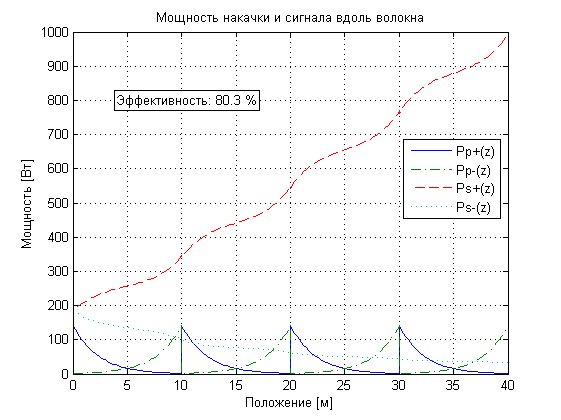
\includegraphics[scale=0.6]{laser_vlrn_3}
  \caption{Мощность накачки и сигнала как функции положения вдоль волокна, рассчитанные с помощью метода <<simple shooting>>.}
  \label{img:laser_vlrn_3}
\end{figure}

Он также находится в хорошем согласии с результатами работы [14]. Расчётная выходная мощность четырехкаскадного ВЛРН составила 963 Вт (в [14] 932 Вт, разница 3 \%), квантовая эффективность лазера при этом равна 80,3 \% (в [14] 77,7 \%). Причина разницы в результатах видится в ошибке, содержащейся в работе [14], так как из приведенного в [14] графика видно, что выходная мощность должна быть по величине больше 950 Вт. Число 932 получается, если ошибочно два раза вычесть отраженный от выходного зеркала сигнал из величины мощности в прямом направлении (в нашем случае получилось бы 931 Вт).

Для проверки корректности получаемых результатов программа была переписана для канонического случая односекционного лазера с зеркалами. Для сравнения результатов мы воспользовались расчетом, приведенным в статье [16]. Использованные в работе параметры приведены в таблице 2.

Таблица 2. Значения параметров, использованных в расчете [16].

Полученный в [16] график зависимости мощности излучения лазера и накачки от длины резонатора приведен на рис. 4. Для сравнения мы взяли случай волокна без потерь.

\begin{figure}[ht]
  \centering
  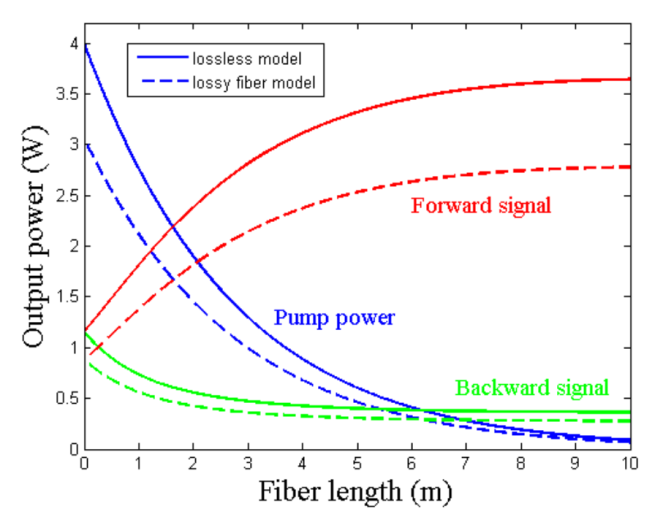
\includegraphics[scale=1.2]{laser_vlrn_4}
  \caption{Распределение мощности сигнала и накачки вдоль волокна при накачке 4 Вт для случая волокна с потерями (пунктирная линия) и без потерь (сплошная линия) [16].}
  \label{img:laser_vlrn_4}
\end{figure}

\begin{figure}[ht]
  \centering
  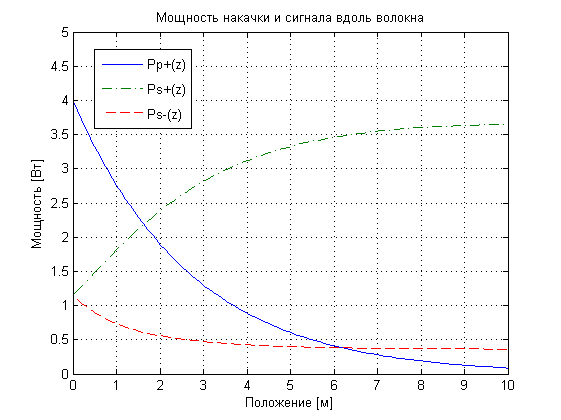
\includegraphics[scale=0.6]{laser_vlrn_5}
  \caption{Распределение мощности сигнала и накачки вдоль волокна при накачке 4 Вт для случая волокна без потерь.}
  \label{img:laser_vlrn_5}
\end{figure}

Полученный результат свидетельствует о корректности нашего расчета.

\section{Оценка пороговых значений киловаттного лазера}

Здесь оценки

% Для расчёта выходной мощности задающего генератора лазера использовался метод, предложенный в [2].
%
% Динамика населенности уровней $n_2$ и $n_1$ описывается скоростными уравнениями. В стационарном случае они упрощаются, и населенность верхнего подуровня может быть записана в виде [2]:
%
% $$n_2=n_1  (Г_р σ_ap λ_p (P_p^++P_p^-)+Г_s σ_as λ_s (P_s^++P_s^-))/(Ahc/τ+Г_р (σ_ap+σ_ep ) λ_p (P_p^++P_p^-)+Г_s (σ_as+σ_es)λ_s (P_s^++P_s^-))                 $$
% (1)
%
% Часть мощности излучения накачки, которая перекрывается с сердцевиной, описывается фактором перекрытия $Г_р$, в первом приближении равном отношению площадей сердцевины и первой оболочки. Соответствующий фактор перекрытия для генерации - $Г_s$ определяется долей мощности лазерной генерации, распространяющейся по сердцевине,  $P_p^+$ и $P_p^-$ - мощности излучения накачки, $P_s^+$ и $P_s^-$ - мощности излучения генерации (знаки плюс и минус соответствуют положительному и отрицательному направлению распространения), $σ_ap$, $σ_ep$ - сечения поглощения и излучения для накачки, $σ_as$, $σ_es$ - сечения поглощения и излучения для генерации, $τ$ - время жизни иона на верхнем лазерном уровне,   - постоянная Планка, $c$ - скорость света в вакууме,  $A$ – площадь поперечного сечения сердцевины, $λ_p$ и $λ_s$ - длины волн накачки и генерации.
%
% Уравнения для описания динамики мощностей накачки и генерации имеют вид [3]:
% $$(dP_p^±)/dz=±Г_р (σ_ap n_0-(σ_ap+σ_ep)n_2 ) P_p^±∓α_p P_p^±$$
% (1)
% $$(dP_s^±)/dz=±Г_s ((σ_as+σ_es)n_2-σ_as n_0 ) P_s^±∓α_s P_s^±$$
% (2)
% где $n_0$ - полное число ионов в единице объема, а $α_p$ и $α_s$ - коэффициенты серых потерь для излучения накачки и генерации.
%
% Граничные условия для уравнений (2) и (3):
% $$P_p^+ (0)=P_pump^+$$
% (4)
% $$P_p^- (L)=P_pump^-$$
% (5)
% $$P_s^+ (0)=R_1 P_s^- (0)$$
% (6)
% $$P_s^- (L)=R_2 P_s^+ (L)$$
% (7)
% $P_pump^+$ и $P_pump^-$ - введенная мощность накачки с каждого из концов (в данном случае вводится только $P_pump^+$), $L$ - длина активной среды, $R_1$ и $R_2$ - эффективные коэффициенты отражения для излучения на длине волны генерации на левом и правом концах резонатора соответственно.
%
% Решение уравнений (1) – (7) может быть найдено с помощью численных методов. Для решения системы дифференциальных уравнений использован метод Рунге-Кутты [2], а также метод стрельбы [2, 3] для поиска неизвестных начальных условий из известных граничных условий.
% \begin{figure}
%   \centering
%   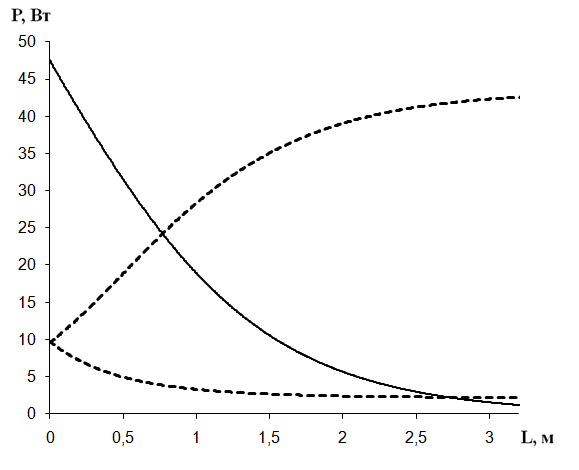
\includegraphics[scale=0.6]{kw-4}
%   \caption{Распределение мощности накачки (сплошная линия) и генерации (пунктирная линия). Выходная мощность: 40,4~Вт. Непоглощенная накачка: 1,18~Вт.}
%   \label{img:kw-4}
% \end{figure}
%
% Результаты расчетов представлены на рисунке 4. Моделирование проводилось при следующих параметрах: L=3,2 м,〖 P〗_pump^+=47,5~Вт,〖 Г〗_р=0.0064,〖 Г〗_s=1,σ_ap= 1.4*〖10〗^(-24)  м^2,σ_ep=1.5*〖10〗^(-24)  м^2,σ_as=3.1*〖10〗^(-28)  м^2,σ_es=0.049*〖10〗^(-24)  м^2,λ_p=975~нм,λ_s= 1080~нм,α_p= 0,02 Дб/м,〖 α〗_s= 0,02  Дб/м,n_0= 1,5*〖10〗^26  1/м^3 ,τ= 800 мкс,A=78.5*〖10〗^(-12)  м^2,R_2= 5~\%,R_1= 99~\%
% \begin{figure}
%   \centering
%   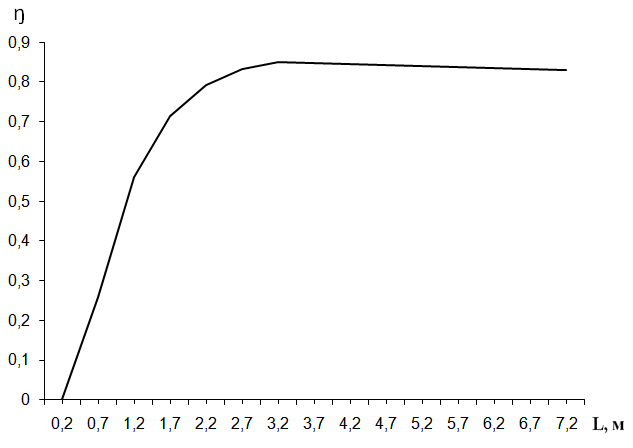
\includegraphics[scale=0.6]{kw-5}
%   \caption{Зависимость эффективности задающего генератора от длины волокна.}
%   \label{img:kw-5}
% \end{figure}
%
% Эффективность задающего генератора с приведенными выше параметрами в зависимости от длины волокна представлена на рисунке 5. Для указанных параметров оптимальная длина составляла 3,2~м. При этом КПД достигает 85~\%. Здесь не учитываются серые потери, потери на сварках и потери из-за не согласованности волокон. Проведенный расчет эффективности показывает качественную оценку оптимальной длины волокна, на практике же эффективность составляет около 70~\%.
%
% Для описания дальнейшего усиления сигнала применяются уравнения (1) – (3), дополненные начальными условиями:
% $$P_p^+ (0)=P_pump^+$$
% (8)
% $$P_s^+ (0)=P_signal^+$$
% (9)
% P_signal^+ - введенная мощность сигнала.
% \begin{figure}
%   \centering
%   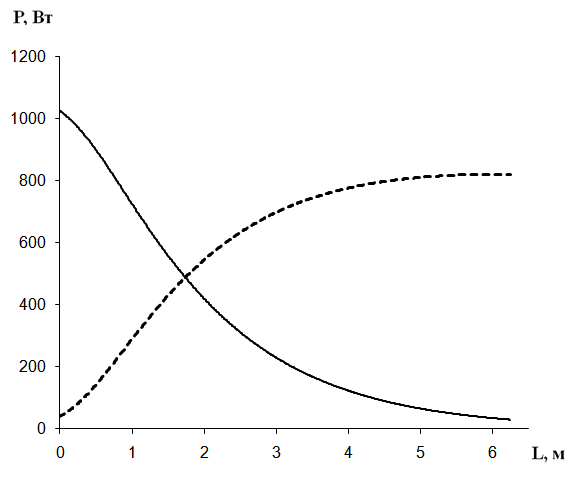
\includegraphics[scale=0.6]{kw-6}
%   \caption{Распределение мощности накачки (сплошная линия) и сигнала (пунктирная линия). Выходная мощность: 821,6~Вт. Непоглощенная накачка: 24.9~Вт.}
%   \label{img:kw-6}
% \end{figure}
%
% На рисунке 6 приведены результаты моделирования усилителя с параметрами: L=6,5 м,P_pump^+=1026  Вт,〖 Г〗_р=0.0025,〖 Г〗_s=1,σ_ap= 1.4*〖10〗^(-24)  м^2,σ_ep=1.5*〖10〗^(-24)  м^2,σ_as=3.1*〖10〗^(-28)  м^2,σ_es=0.049*〖10〗^(-24)  м^2,λ_p=975~нм,λ_s= 1080~нм,α_p= 0,02 Дб/м,〖 α〗_s= 0,02  Дб/м,n_0= 1,8*〖10〗^26  1/м^3 ,τ= 800 мкс,A=314*〖10〗^(-12)  м^2,P_signal^+=40,4~Вт
%
% \begin{figure}
%   \centering
%   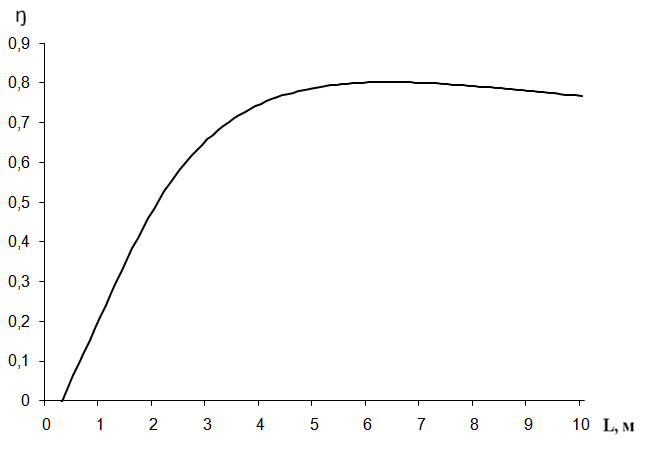
\includegraphics[scale=0.6]{kw-7}
%   \caption{Зависимость эффективности усилителя от длины волокна.}
%   \label{img:kw-7}
% \end{figure}
%
% Эффективность смоделированного усилителя в зависимости от длины волокна представлена на Рисунке 7. Для указанных параметров оптимальная длина составила 6,5 м. При этом КПД достигает 80%.

\section{Изготовление основных узлов и компонентов}
\label{sec:kw-manufacturing}

\subsection{Система электропитания лазера}

Изготовленная система электропитания лазера может обеспечить питанием 301 лазерный модуль накачки и позволяет управлять выходной мощностью лазера. Электропитание лазера осуществляется от сети 380 В. Ток на модули накачки подается стабилизированными преобразователями напряжения. Система электропитания рассчитана на потребление до 46~кВт. Структурная схема системы электропитания приведена на рисунке 8.
\begin{figure}
  \centering
  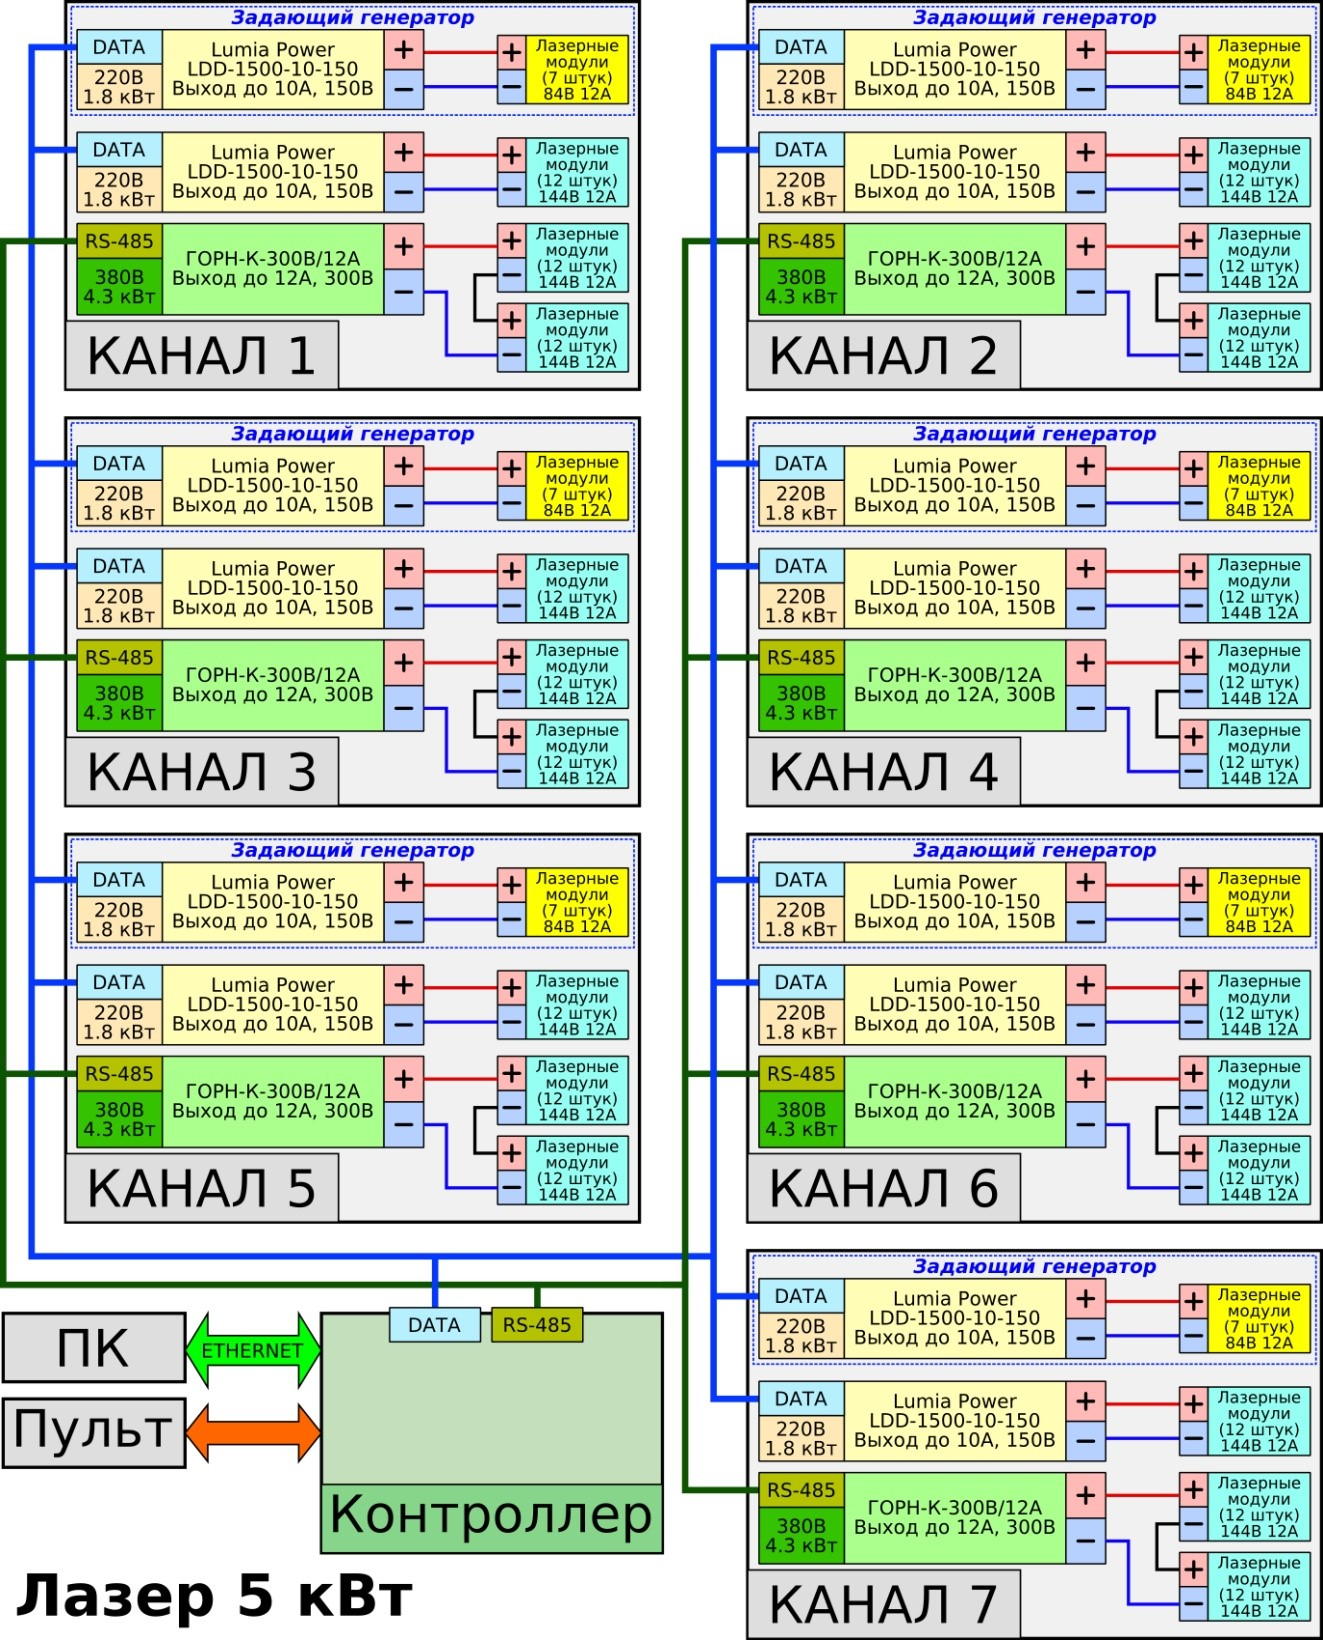
\includegraphics[scale=0.6]{kw-8}
  \caption{Структурная схема системы электропитания.}
  \label{img:kw-8}
\end{figure}

\subsection{Система охлаждения лазера}

Для обеспечения эффективного теплоотвода модули накачки располагаются на плитах Р56-Л2641.110 и Р56-Л2641.220. В плитах просверлены каналы для обеспечения водяного охлаждения. Каждый лазерный канал содержит три охлаждаемые водой плиты. Охлаждение и циркуляция воды обеспечивается внешним чиллером. Распределение воды на каналы осуществляется специально разработанным коллектором Р56-Л2641.300. Необходимый расход воды обеспечивается четырьмя насосами. Изображения плит и коллектора представлено на рисунках 9, 10 и 11.
\begin{figure}
  \centering
  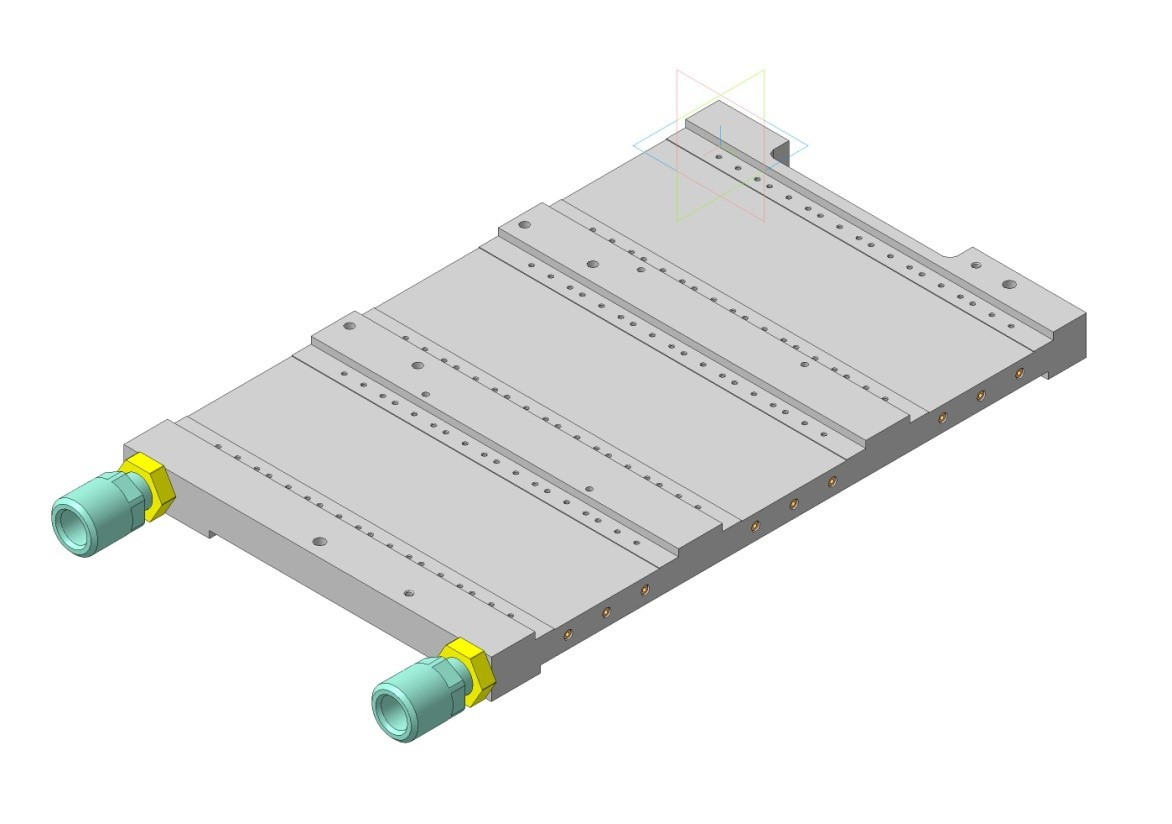
\includegraphics[scale=0.6]{kw-9}
  \caption{Плита Р56-Л2641.110.}
  \label{img:kw-9}
\end{figure}
\begin{figure}
  \centering
  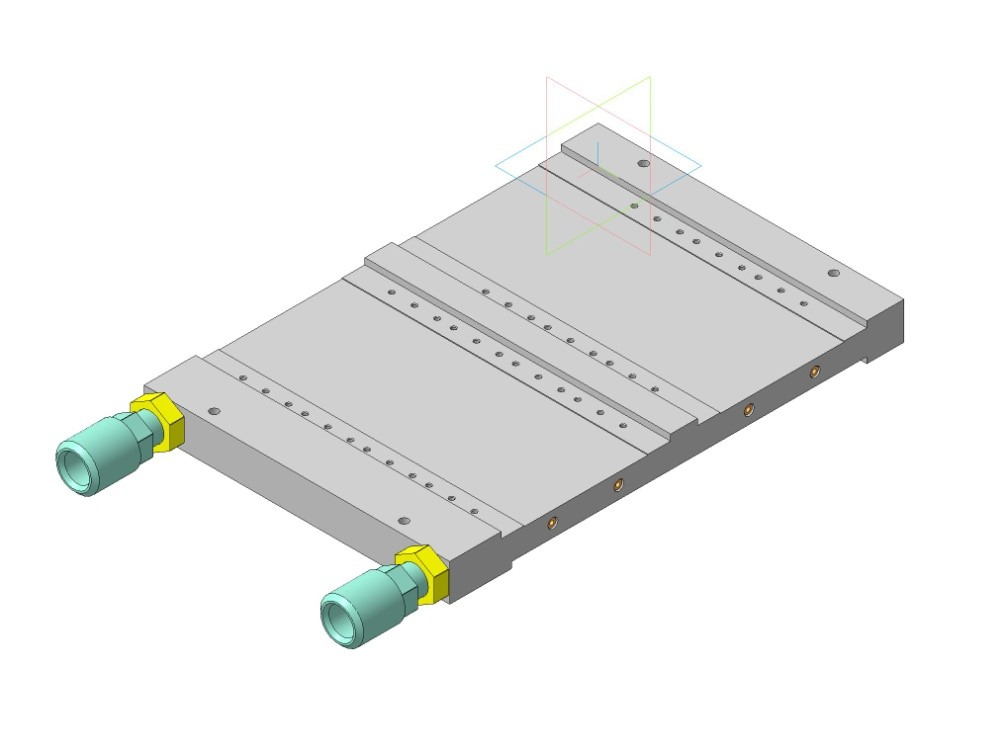
\includegraphics[scale=0.6]{kw-10}
  \caption{Плита Р56-Л2641.220.}
  \label{img:kw-10}
\end{figure}
\begin{figure}
  \centering
  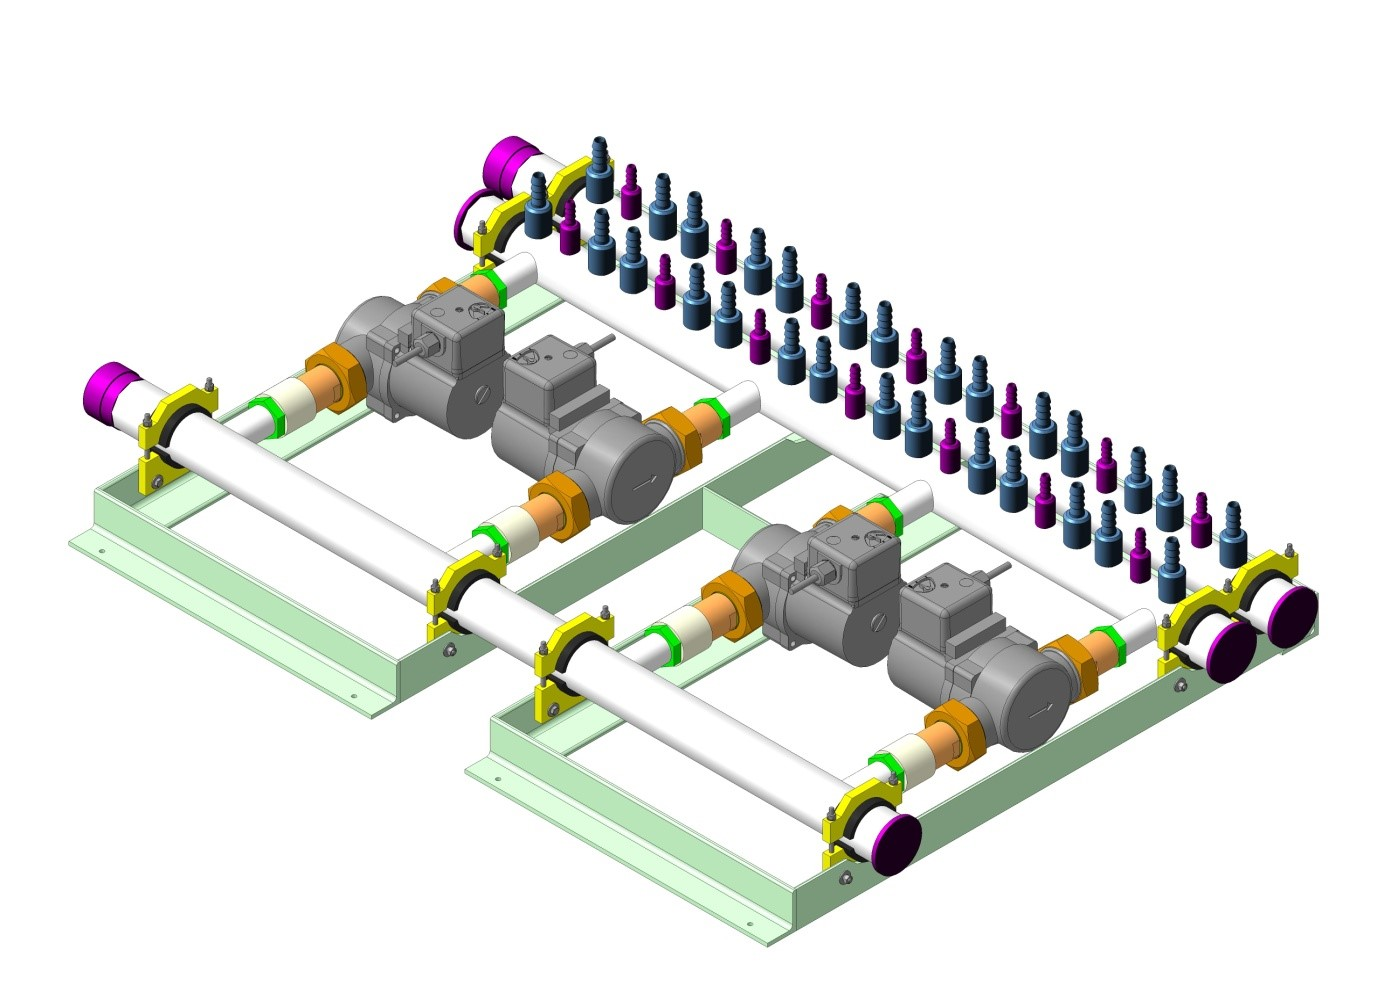
\includegraphics[scale=0.6]{kw-11}
  \caption{Коллектор Р56-Л2641.300.}
  \label{img:kw-11}
\end{figure}


\subsection{Изготовление модулей накачки}

По результатам разработки и изготовления модулей накачки были выпущены: протокол 057-04/5948 от 18.09.15 [4] «Изготовление модулей накачки ОВЛДН 5..10~кВт»; отчет о НИР ПС15.13802/2 «Проведение исследований в интересах …» [5].
На рисунке 12 представлена типичная ватт-амперная характеристика модуля накачки.
\begin{figure}
  \centering
  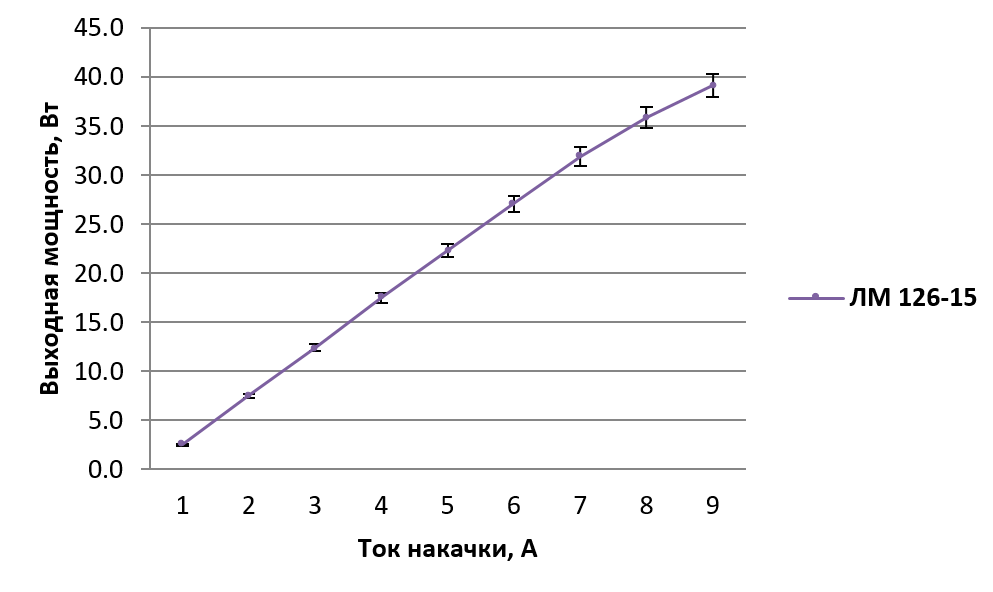
\includegraphics[scale=0.6]{kw-12}
  \caption{Типичная ватт-амперная характеристика модуля накачки.}
  \label{img:kw-12}
\end{figure}

Внешний вид модуля накачки представлен на рисунках 13 и 14.
\begin{figure}
  \centering
  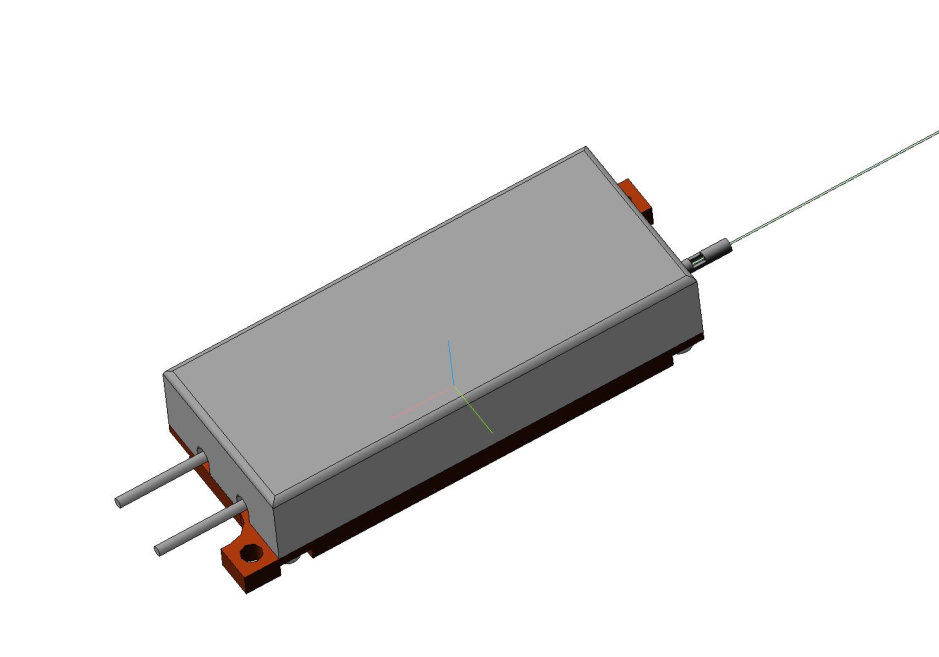
\includegraphics[scale=0.6]{kw-13}
  \caption{Внешний вид модуля накачки.}
  \label{img:kw-13}
\end{figure}
\begin{figure}
  \centering
  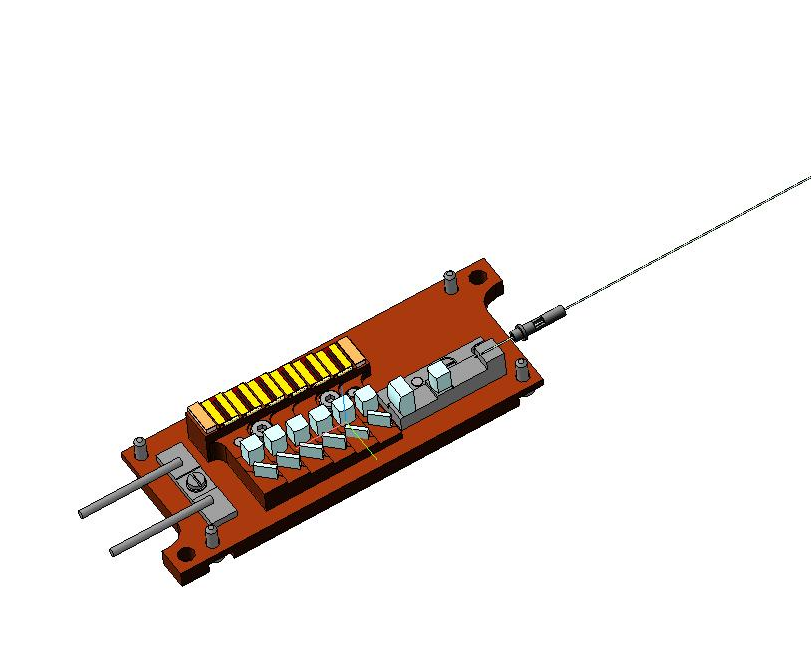
\includegraphics[scale=0.6]{kw-14}
  \caption{Внешний вид модуля накачки без крышки.}
  \label{img:kw-14}
\end{figure}


\subsection{Задающий генератор}

\begin{figure}
  \centering
  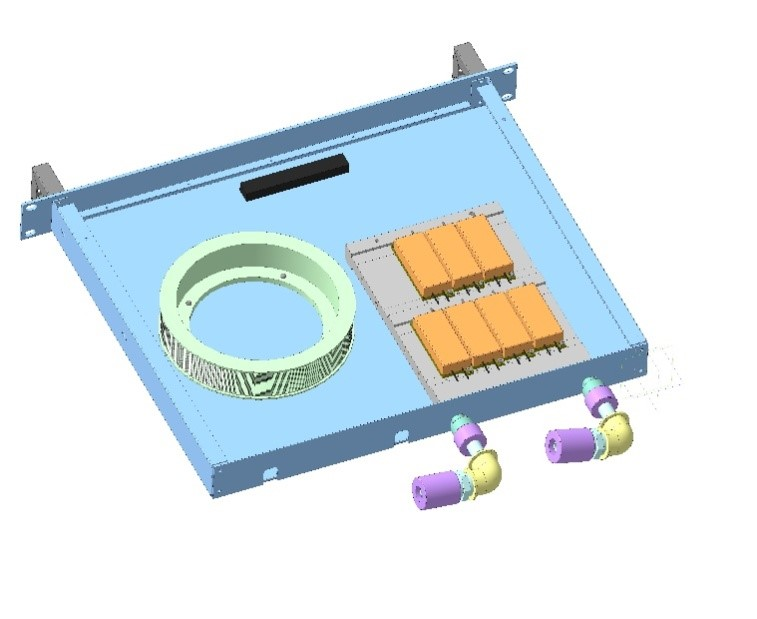
\includegraphics[scale=0.6]{kw-15}
  \caption{Теплоотвод, каплер и катушка в корпусе задающего генератора.}
  \label{img:kw-15}
\end{figure}

В ЭЦ НИО-5 согласно КД Р56-Л2641 изготовлены внутренние элементы (теплоотводы, катушки) и доработан корпус задающего генератора. Для обеспечения теплоотвода активного волокна была разработана и изготовлена катушка КД Р56-Л2641.201
\begin{figure}
  \centering
  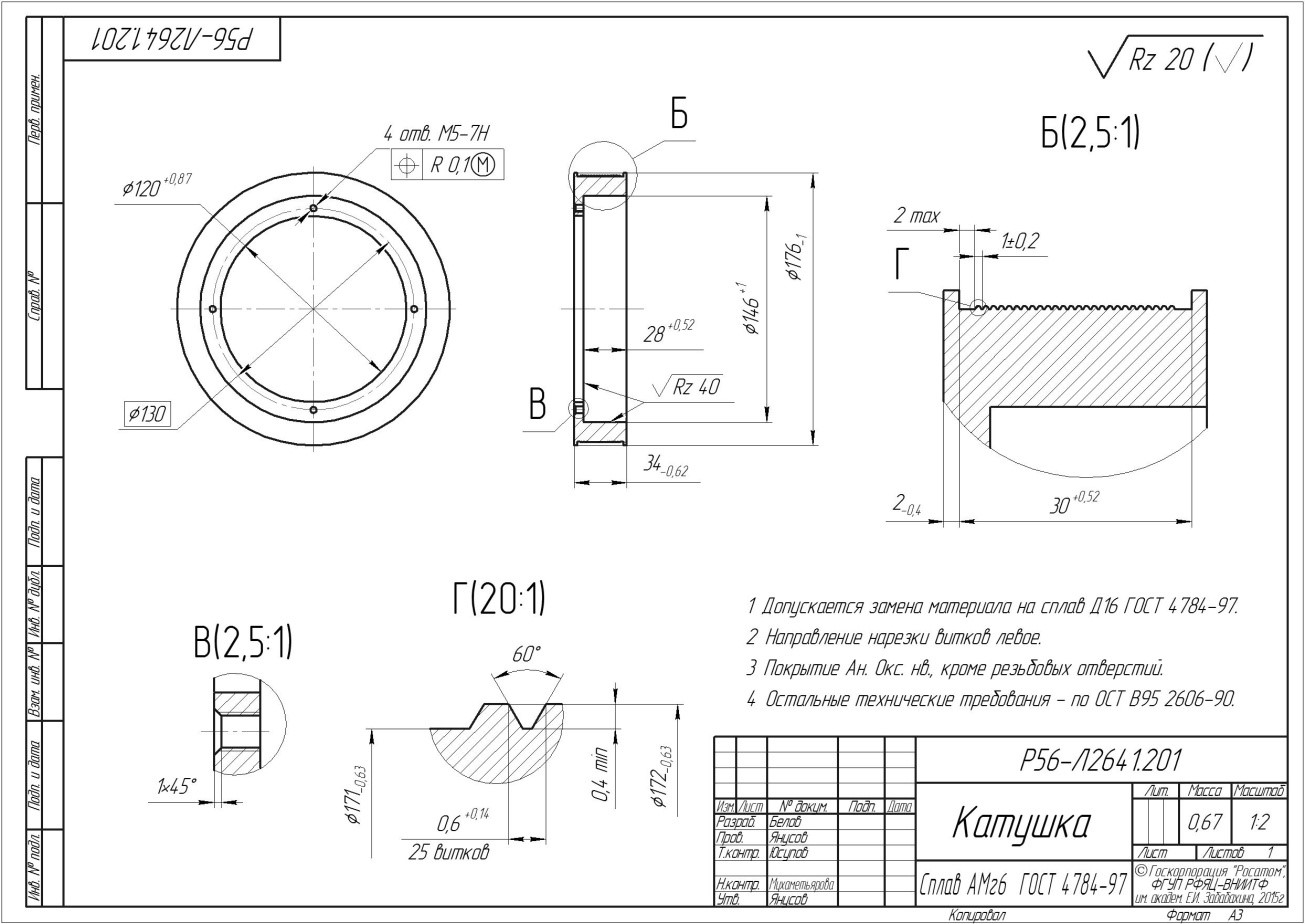
\includegraphics[scale=0.6]{kw-16}
  \caption{Катушка для активного волокна задающего генератора.}
  \label{img:kw-16}
\end{figure}


\subsection{Усилитель}

\begin{figure}
  \centering
  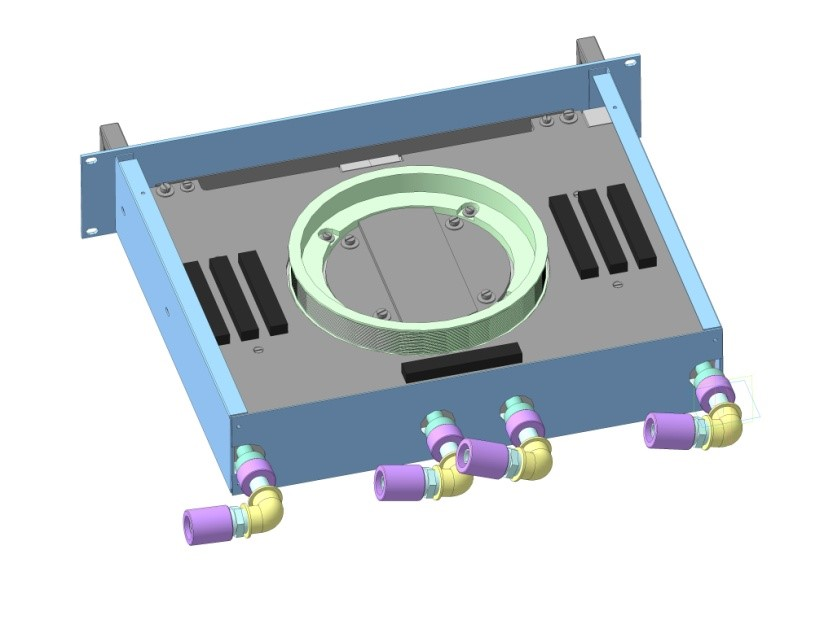
\includegraphics[scale=0.6]{kw-17}
  \caption{Теплоотвод, каплеры и катушка в корпусе усилителя.}
  \label{img:kw-17}
\end{figure}
\begin{figure}
  \centering
  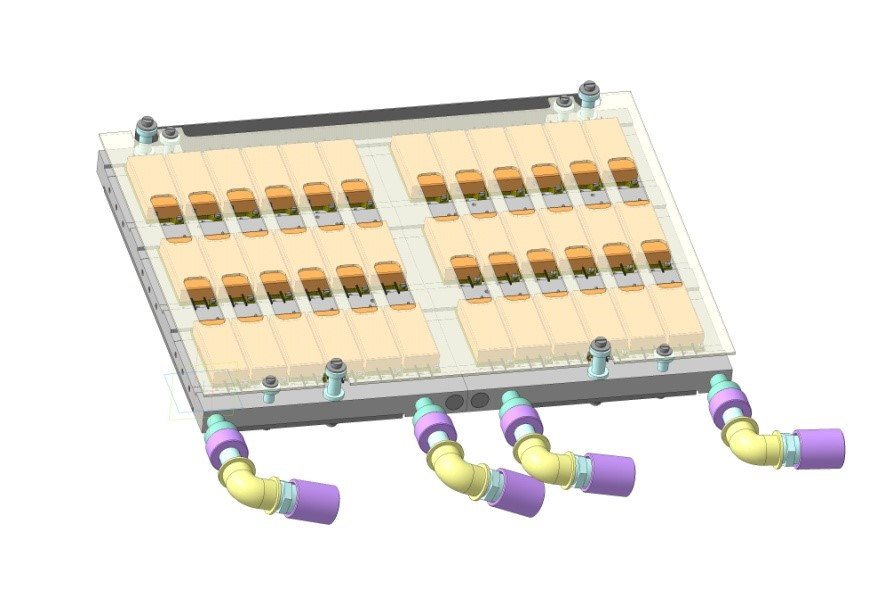
\includegraphics[scale=0.6]{kw-18}
  \caption{Модули накачки на теплоотводе в корпусе усилителя.}
  \label{img:kw-18}
\end{figure}

В ЭЦ НИО-5 согласно КД Р56-Л2641 изготовлены внутренние элементы (теплоотводы, катушки) и доработан корпус усилителя. Для обеспечения теплоотвода активного волокна была разработана и изготовлена катушка КД Р56-Л2641.103
% \begin{figure}
%   \centering
%   \includegraphics[scale=0.6]{kw-}
%   \caption{Катушка для активного волокна усилителя.}
%   \label{img:kw-}
% \end{figure}

\section{Сборка и экспериментальная отработка лазера}
\label{sec:kw-assembly}

Накачка активного волокна осуществлялась модулями накачки мощностью примерно 30-35~Вт производства ВНИИТФ. Типичный спектр излучения модуля при токе 8~А показан на рисунке 20.
\begin{figure}
  \centering
  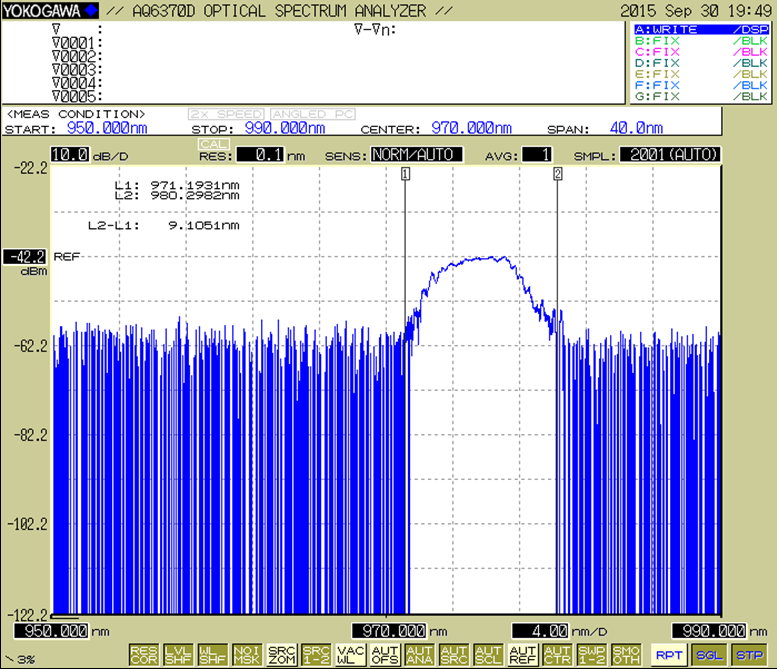
\includegraphics[scale=0.6]{kw-20}
  \caption{Типичный спектр модуля накачки.}
  \label{img:kw-20}
\end{figure}

Как видно из рисунка 20 ширина спектра модуля по основанию составляет примерно 9~нм с центром в области 976~нм, что удовлетворяет требованиям по накачке активного волокна.

Согласно проведенному расчету длина активного волокна ЗГ должна составлять 3,2 м, поэтому изначально была отмерена указанная длина, и волокно было намотано на теплоотводящую катушку. После чего к активному волокну были подварены волоконные брэгговские решетки и каплер, как показано на рисунке 1. В итоге выходная мощность ЗГ составила примерно 36~Вт при введенной мощности накачки 50~Вт, что соответствует эффективности преобразования <<свет в свет>> 72~\%. Для ЗГ было использовано 2 модуля накачки.

Оптимальная длина волокна для усилителя составляет примерно 7 м. Указанная длина волокна была намотана на теплоотводящую катушку. Для накачки активного волокна использовалось 36 модулей накачки, которые были расположены на теплоотводе. Модули накачки подваривались к каплеру  типа (6+1)х1 через каплер типа 7х1 как показано на рисунке 3. Суммарная мощность накачки составила примерно 1000~Вт. Мощность усиленного сигнала составила примерно 800~Вт. Учитывая, что мощность излучения ЗГ составляла 36~Вт, то в усилителе было запасено 764~Вт. Эффективность преобразования «свет в свет» составила 76%.
\begin{figure}
  \centering
  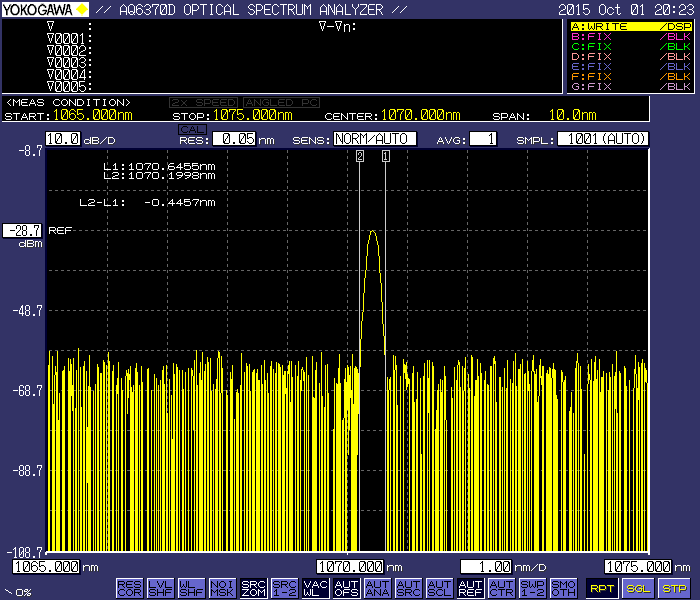
\includegraphics[scale=0.6]{kw-21}
  \caption{Спектр генерации.}
  \label{img:kw-21}
\end{figure}

На рисунке 21 приведен спектр генерации при токе накачки 8 А. Видно, что в спектре генерации составляющие люминесценции отсутствуют. Ширина спектра составила примерно 0,5~нм по основанию.

Мощность излучения более 5~кВт достигается путем объединения семи аналогичных лазерных каналов. Для этого семь выходных волокон лазерных каналов помещаются в капилляр и в металлическую трубку для теплоотвода. Торец выходной части лазера представлен на рисунке 22.
\begin{figure}
  \centering
  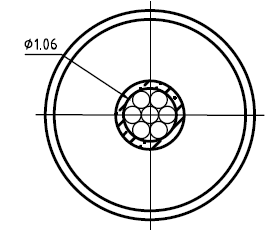
\includegraphics[scale=0.6]{kw-22}
  \caption{Выходная часть лазера.}
  \label{img:kw-22}
\end{figure}

Особое место при сборке мощного ОВЛДН следует уделять сварке волокон, поскольку неточные параметры сваривания или геометрические рассогласования волокон приводят к увеличению потерь на стыке волокон, а следовательно и к ограничению максимальной мощности лазера. Поэтому необходимо оптимизировать углы скола волокон, напряжение волокна, время сварки и мощность дуги или нагревателя. Восстанавливающий покрытие материал должен минимально возможно рассеивать излучение.
Скол волокна в настоящей работе выполнялся с помощью скалывателя Vytran LDC-400, а сварка волокон выполнялась с помощью сварочного аппарата Fujikura FSM-100P.

\section{Заключение}
\label{sec:kw-conclusion}

Проведена разработка лабораторного образца лазера, в ходе которой решены основные научно-технические проблемы, стоящие на пути создания мощных ОВЛДН (излучаемой мощностью 5..10~кВт): разработана оригинальная конструкция модулей накачки высокой яркости (плотность мощности 6 МВт/см2 ср) на отечественной элементной базе, освоено их изготовление с производительностью 2 модуля в смену; разработана оптическая схема лазера, проведена отработка критических узлов; разработана оригинальная система охлаждения лазера, позволяющая снизить требования к внешнему контуру охлаждения.

Разработана КД Р56-Л2641 на лабораторный образец лазера, проведено его изготовление и экспериментальная отработка. Исходя из существующих на настоящий момент технологий, мощность излучения 5~кВт, обеспечивается путем объединения излучения семи лазерных модулей с мощностью 800~Вт. При этом энергопотребление лазера без внешнего контура системы охлаждения составляет $\approx$ 25~кВт (КПД 20~\% <<от розетки>>).

Отработанные в ходе работы схемные и технические решения позволяют создавать непрерывные оптоволоконные лазеры с выходной мощностью до 10~кВт, заложены научно-технические основы для дальнейшего увеличения мощности оптоволоконных лазеров.

%%%-----------------------------------------------------------------------------

\clearpage
